\documentclass[12pt, a4paper, oneside]{ctexart}
\usepackage{fancyhdr}
\usepackage{amsmath, amsthm, amssymb, bm, graphicx, hyperref, mathrsfs, graphicx, float, subfigure, caption, makecell, longtable,framed}
\usepackage[dvipsnames]{xcolor}
\usepackage{listings}
\usepackage{indentfirst}
\usepackage{labels}
\setlength{\parindent}{2em}
\renewcommand{\lstlistingname}{code}
\lstset{
    language=C, % 设置语言
 basicstyle=\ttfamily, % 设置字体族
 breaklines=true, % 自动换行
 keywordstyle=\bfseries\color{NavyBlue}, % 设置关键字为粗体,颜色为 NavyBlue
 morekeywords={}, % 设置更多的关键字,用逗号分隔
 emph={self,input,output,wire,reg,posedge,negedge}, % 指定强调词,如果有多个,用逗号隔开
    emphstyle=\bfseries\color{Rhodamine}, % 强调词样式设置
    commentstyle=\itshape\color{black!50!white}, % 设置注释样式,斜体,浅灰色
    stringstyle=\bfseries\color{PineGreen!90!black}, % 设置字符串样式
    columns=flexible,
    numbers=left, % 显示行号在左边
    numbersep=2em, % 设置行号的具体位置
    numberstyle=\footnotesize, % 缩小行号
    frame=single, % 边框
    framesep=1em % 设置代码与边框的距离
}
\usepackage[left=1in, right=1in, top=1in, bottom=1in]{geometry}


\ctexset{
    % 修改 section。
    section={   
        format=\heiti\raggedright\zihao{-2} % 设置 section 标题为黑体、右对齐、小4号字
    },
    % 修改 subsection。
    subsection={   
        format=\heiti\zihao{4} % 设置 subsection 标题为黑体、5号字
    }
}


\pagestyle{fancy}
\fancyhf{}
\renewcommand{\headrulewidth}{0pt}
\fancyfoot[C]{\thepage}

\title{\textbf{8086实验报告}}
\author{张浩宇 522031910129}
\date{}

\begin{document}
    \maketitle
    \section{实验一 I/O译码}
    \subsection{读入开关状态并输出}
    \begin{figure}[!h]
        \centering
        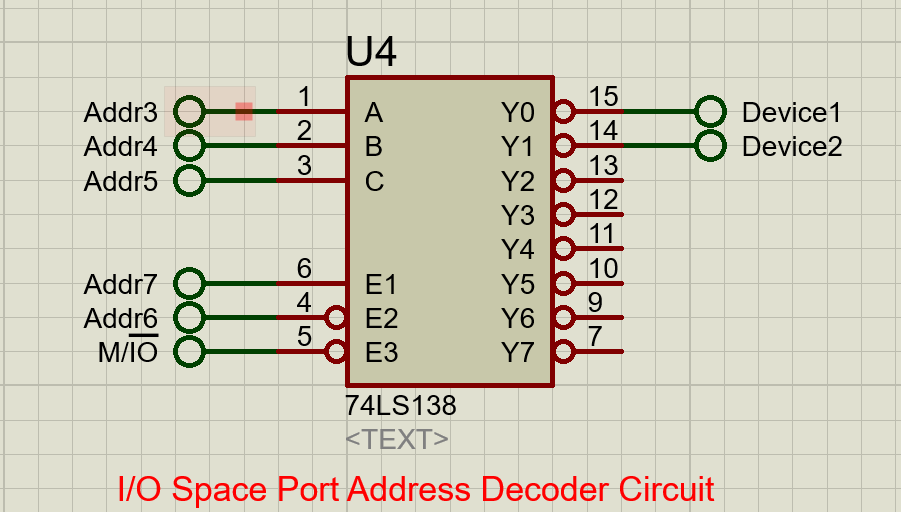
\includegraphics[width=0.8\textwidth]{img/fig1-183decoder.png}
        \caption{I/O译码电路}
        \label{fig:decoder}
    \end{figure} 
    输入口(74LS244)和输出口(74LS273)的片选端口分别为Device1和Device2,通过74LS138进行IO地址译码,如图{\ref{fig:decoder}}。
    当Device1为低电平,选中74LS244,即为输入;当Device2为低电平,选中74LS273,即为输出。根据译码器连接方式,输入端口地址80H,输出端口地址88H。
    
    因此从输入端口读入开关状态,取反输出到输出端口,即可实现开关状态的读入和输出。
    \subsection{模拟交通灯}
    如图,交通灯为6个分为2组的共阳级LED,其另一端接在74LS273输出端口,
    当对应位输出低电平时,LED亮,则每一种亮灯状态对应一个8位编码,将该编码
    从74LS273的端口地址输出就可以按照对应状态点亮LED。

    代码的运行是很快的,为了让亮灯的效果保持以便看清,需在改变LED状态后进行延时操作以保留。
    延时等待的效果可以通过循环重复多次操作实现。由于程序中需多次进行延时,可以将延时程序
    写为一个子过程,在需要时调用。

    该程序可以看作一个状态机,每个状态对应一段包括输出LED编码、延时、状态跳转的操作。从初始状态进入后,
    在不同状态之间循环,实现交通灯的模拟。

    要实现灯闪烁的效果可以通过在LED的亮和灭的状态中快速切换实现,多次切换的过程可以通过
    循环语句完成。在切换中也需要短时间的延时才能看清变化。
    \subsection{修改选片地址}
    在该电路中,74LS244和74LS273的片段端口分别为Device1和Device2,这两个端口连接在译码器的输出端,而地址总线连接在译码器的
    输入端,输入地址决定译码器的哪个输出口为低电平从而使能I/O端口芯片。因此改变Device1和Device2的在译码器上的位置就可以改变
    对应的片选地址。要改为,只需把,如图。

    要在修改选片地址后完成开关状态的写入和输出,只需将源代码中的输入和输出端口地址修改为新的地址即可。

    \subsection{实验中的问题与解决}
    在编写延时程序时,通过一层LOOP循环实现延时,但是在实际运行中发现延时时间不够长,LED状态切换过快。
    在一层LOOP循环中在添加一层由跳转语句控制的第二层循环后,延时时间变长,效果符合预期。
    \section{内存扩展和I/O空间操作}
    \subsection{8255接口操作}
    \subsubsection{8255在I/O空间的地址}
    8255的$\overline{\text{CS}}$为引脚,为低电平时8255才工作,其连接在译码器Y2,由地址Addr7-Addr3控制,如图。
    要选片8255,Addr7-Adddr3应为10010。
    此外8255的A、B、C三个口和控制寄存器的选择由A1、A0决定,分别由Addr2、Addr1控制。8255使用低8为数据线,
    对应偶地址,Addr0为0。因此8255的地址分别为:

    A(A1A0=00):10010000B=90H

    B(A1A0=00):10010010B=92H

    C(A1A0=00):10010100B=94H

    控制寄存器(A1A0=00):100010110B=96H
    \subsubsection{接收输入并通过数码管和LED输出}
    根据8255连接方式,如图,A口高4位连接LED,A口低4位连接数码管位选,B口连接数码管段选,
    C口连接开关输入。故应该将8255设置为方式0,A口为输出,B口为输出,C口为输入,对应控制字10001001B。

    将控制字输出至8255的控制寄存器完成8255的初始化,然后通过C口读入开关量,取其高4位并将低4位变为1110B
    输出至A口实现LED显示和数码管位选,根据低4位输出段码至B口实现数码管段选。在输出段码时,可预先将1-F的段码
    存储在数据段,输出时根据相应的值寻址并取出。


    \subsubsection{接收输入并通过多位数码管输出}
    该实验8255连接和初始化配置与上个实验相同。由于需要数码管多位显示不同的数字,而数码管同时
    只能接收一个段码的输入,因此需要在数码管的显示周期内快速切换显示的段码和位选,以实现多位显示。

    \subsubsection{实验中的问题与解决}
    \paragraph{(1)} 在进行I/O操作时,由于输入和输出只能通过AX/AL寄存器进行,直接操作输入量会被覆盖。
    应当在输入后保存输入量以便进行多次操作。

    \paragraph{(2)} 在该实验中需要对一个寄存器进行移位SHR右移4位,
    但直接 SHR AL,4会报错,因为用立即数来移位只能移动1位,移动多位
    应当先在一个寄存器中保存移位值,再进行移位操作。

    \paragraph{(3)} 在通过快速切换段码和位选来实现数码管多位显示不同数字时,
    会出现显示乱码的情况。这是因为切换过快导致重叠,因此应该在切换之间加上短时间的延迟。


    

    \subsection{内存扩展}
    \subsubsection{内存地址和大小}
    根据原理图中内存地址译码部分和内存芯片部分,如图,内存由两片32KB的芯片组成,为U10和U11,分别对应偶地址和奇地址。
    总的内存容量为64KB。根据地址译码电路,当Addr19-Addr16为0100B时,Y4为0,能选中内存芯片,Addr15-Addr1为片内地址,
    Addr0在U10和U11中选择,决定奇偶地址,故地址范围是40000H-4FFFFH。
    \subsubsection{内存写入}
    已知U10和U11内存范围是40000H-4FFFFH,可将4000H作为段基址,就是对U10和U11进行操作。

    要操作内存,可以通过寄存器相对寻址的方法,将BX寄存器作为偏移地址,AX寄存器存储要放入内存的数值,通过循环,
    每次放入内存并增加寄存器的值,实现对内存的遍历操作。

    当操作完所有内存后,需要结束循环,由于偏移地址寄存器(16bit)的可表示的内存单元数与总的内存容量一致(64K),
    当出现进位时恰操作完,因此进位标志可以作为循环终止的判断条件。

    \subsubsection{实验中的问题与解决}
    \paragraph{(1)} 在该实验中,需要修改段寄存器DS的值,而段寄存器只能通过寄存器寻址方式赋值,不能用立即数寻址。
    \paragraph{(2)} 8086在操作内存时,默认是以字为单位进行操作,因此在本实验需要在代码中指明内存操作数的宽度属性是字节。
    \section{定时器、计数器的应用}

    
\end{document}

